%\chapter{Visualização simultânea de imagens e superfície}
\chapter{Simultaneous viewing of images and surfaces}

%A visualização simultânea de imagens e superfície pode ser acionada clicando com o botão
%\textbf{esquerdo} do mouse sobre o atalho localizado no canto inferior direito da tela do
%InVesalius. Veja a figura \ref{fig:slice_plane_original}.
The simultaneous viewing of images and surfaces can be activated in InVesalius by clicking the left mouse button on the shortcut located in the lower right corner of the InVesalius screen. See figure~ \ref{fig:slice_plane_original}.

\begin{figure}[!htb]
\centering
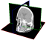
\includegraphics[scale=0.6]{slice_plane_original}
\caption{Shortcut for simultaneous viewing}
\label{fig:slice_plane_original}
\end{figure}

%Este recurso permite habilitar ou desabilitar a exibição das imagens nas diferentes
%orientações (ou planos) na mesma janela de visualização da superfície 3D. Para isso, basta
%marcar ou desmarcar a opção correspondente no menu indicado na figura \ref{fig:view_2d_3d_1}.

This feature allows one to either enable or disable the display of images in different orientations (or plans) within the same display window of the 3D surface. To do this, simply check or uncheck the corresponding option in the menu shown in figure~\ref{fig:view_2d_3d_1}.

\begin{figure}[!htb]
\centering
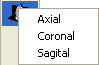
\includegraphics[scale=0.6]{view_2d_3d_1}
\caption{Selection of the guidelines (plans) to display}
\label{fig:view_2d_3d_1}
\end{figure}

%Vale notar que uma orientação, quando selecionada, apresenta uma marca na opção correspondente.
%Isso é ilustrado na figura \ref{fig:view_2d_3d_2}.

It is worth noting when the particular orientation is selected, a check is presented in the corresponding option. This is illustrated in figure~\ref{fig:view_2d_3d_2}.

\begin{figure}[!htb]
\centering
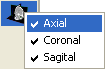
\includegraphics[scale=0.6]{view_2d_3d_2}
\caption{Selected Guidelines for display}
\label{fig:view_2d_3d_2}
\end{figure}


\newpage


%Se a superfície já estiver sendo exibida, os planos das orientações serão apresentados como mostra
%a figura \ref{fig:3d_planes}. Caso contrário, somente os planos serão exibidos
%(figura \ref{fig:only_2d_planes}).

If the surface is already displayed, the plans of the guidelines will be presented as shown in figure~\ref{fig:only_2d_planes}. Otherwise, only the plans will be displayed

\begin{figure}[!htb]
\centering
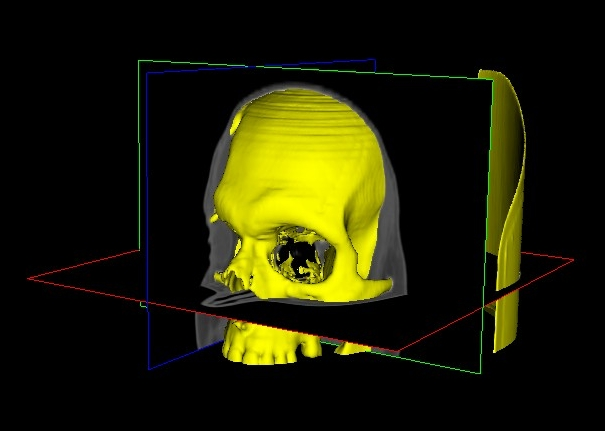
\includegraphics[scale=0.5]{3d_planes}
\caption{Surface and plans displayed simultaneously}
\label{fig:3d_planes}
\end{figure}

\begin{figure}[!htb]
\centering
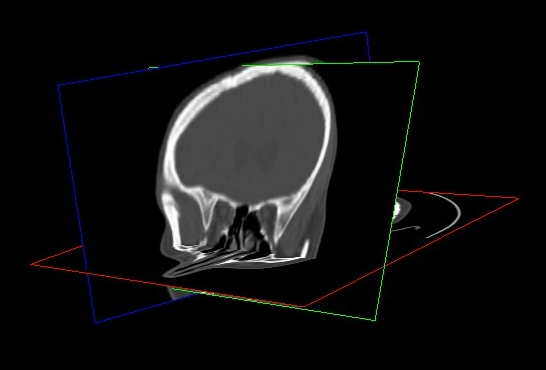
\includegraphics[scale=0.55]{only_2d_planes}
\caption{Flat display (no surface)}
\label{fig:only_2d_planes}
\end{figure}

\newpage

%Para desativar a exibição de um plano, basta desmarcar a opção correspondente no menu
%(figura \ref{fig:view_2d_3d_2}).

To view the display of a plan, just uncheck the corresponding option in the menu (figure~\ref{fig:view_2d_3d_2})